\begin{frame}
  \frametitle{Evaluation: 23K pages budget}
  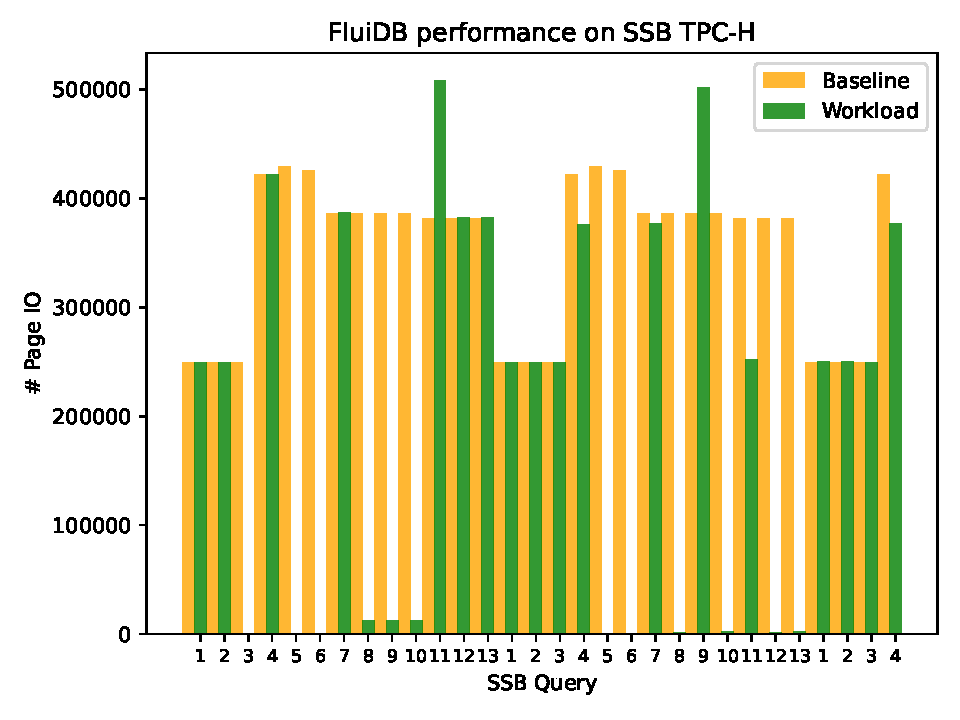
\includegraphics[width=.9\linewidth]{../plans/io_perf_23000.pdf}
\end{frame}

\begin{frame}
  \frametitle{Evaluation: 65K pages budget}
  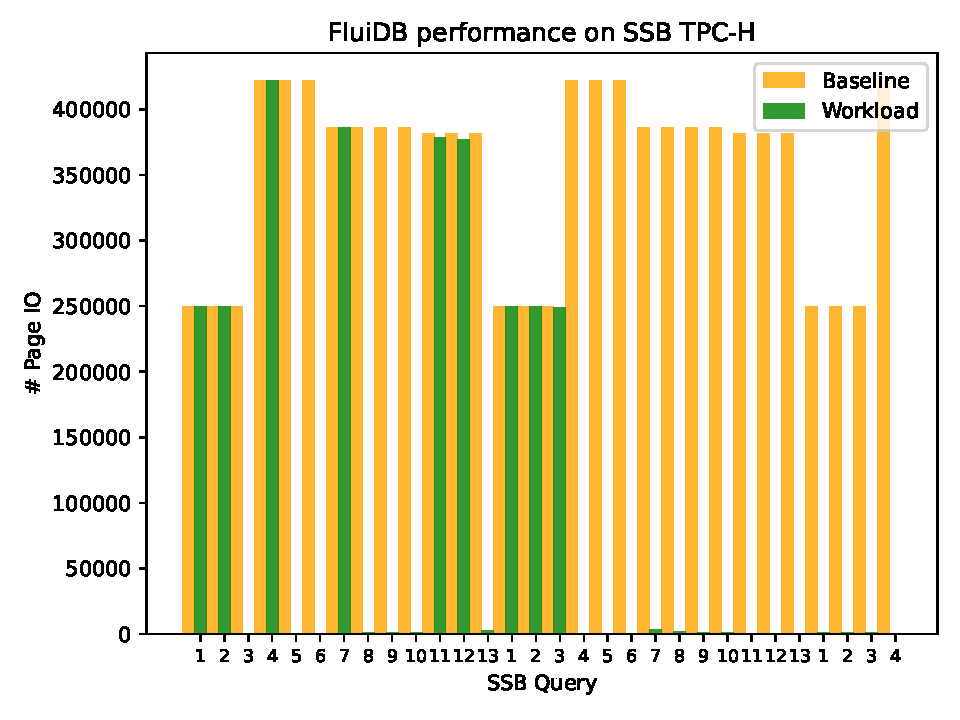
\includegraphics[width=.9\linewidth]{../plans/io_perf_65000.pdf}
\end{frame}

\begin{frame}
  \frametitle{Evaluation: But ... 61K pages budget}
  \framesubtitle{lineorder is deleted at 6 because all join outputs were materialized}
  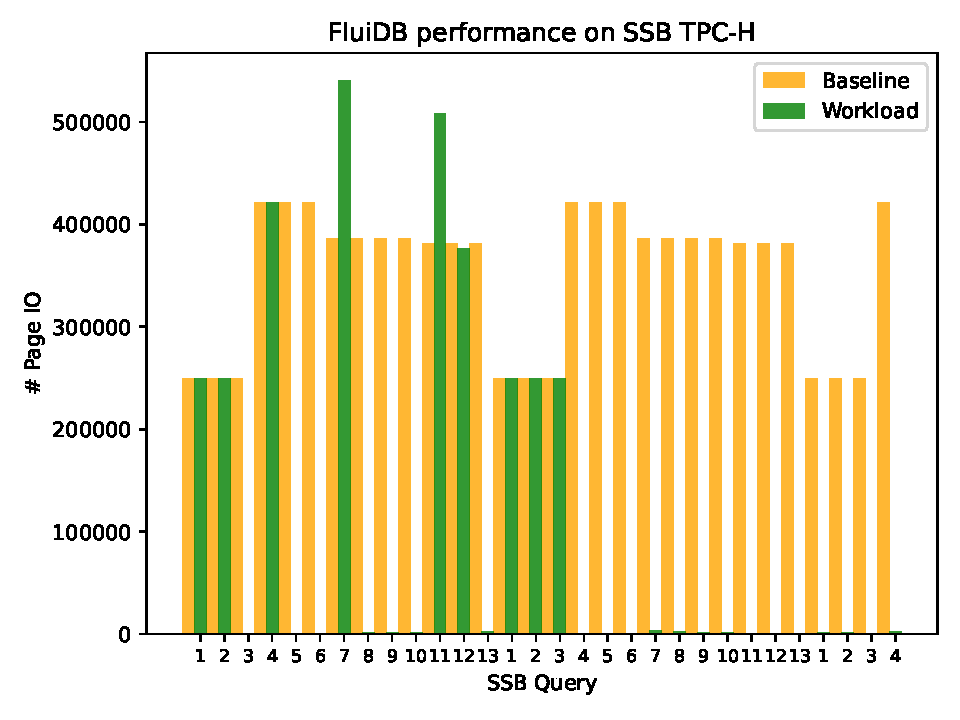
\includegraphics[width=.9\linewidth]{../plans/io_perf_61000.pdf}
\end{frame}

\newcommand\joingr[4]{
  \begin{tikzdiagram_h}
    \tikzset{node distance=4cm}
    \tikzset{nomat/.style={ellipse,draw}}
    \tikzset{mat/.style={ellipse,draw,fill=gray!30}}
    \tikzset{have/.style={ellipse,draw,fill=green!30}}
    \tikzset{need/.style={ellipse,draw,fill=red!30}}
    \tikzset{tnode/.style={rectangle,draw}}

    \node[tnode] (t) {\(\Join\)};
    \node[#3] (o) [above of=t] {\(A_{useful} \Join B\)};
    \node[#4] (a_l) [above left of=t] {\(A_{useful} \lnsemi B\)};
    \node[#4] (a_r) [above right of=t] {\(A_{useful} \rnsemi B\)};
    \node[#2] (i_l) [below left of=t] {\(A_{useful}\)};
    \node[#1] (i_r) [below right of=t] {\(B\)};

    \path (t) edge (o);
    \path (t) edge (a_l);
    \path (t) edge (i_l);
    \path (t) edge (a_r);
    \path (t) edge (i_r);
  \end{tikzdiagram_h}
}


\begin{frame}{Plenty of memory}
  \only<1>{\joingr{mat}{mat}{nomat}{nomat}}
  \only<2>{\joingr{mat}{mat}{mat}{mat}}
  \only<3>{\joingr{mat}{have}{mat}{mat}}
\end{frame}

\begin{frame}{Being on a budget}
  \only<1>{\joingr{mat}{mat}{nomat}{nomat}}
  \only<2>{\joingr{mat}{mat}{mat}{nomat}}
  \only<3>{\joingr{mat}{have}{mat}{nomat}}
\end{frame}

\begin{frame}{Having just enough rope}
  \only<1>{\joingr{mat}{mat}{nomat}{nomat}}
  \only<2>{\joingr{mat}{mat}{mat}{mat}}
  \only<3>{\joingr{nomat}{nomat}{mat}{mat}}
  \only<4>{\joingr{nomat}{need}{mat}{mat}}
\end{frame}
